\subsection{Descripci\'on del problema}

En este punto se nos pide resolver el problema de ubicar centrales de gas de manera estrat\'egica entre los pueblos de una cierta regi\'on.\\

Dados $n$ pueblos con sus respectivas coordenadas en el plano y $k$ centrales de gas, la idea es decidir en qu\'e pueblos ubicar las centrales. Adem\'as es posible construir tuber\'ias entre pueblos: una tuber\'ia que va de un pueblo con central a uno sin no s\'olo transporta el gas a este \'ultimo sino que adem\'as lo convierte en potencial proveedor. Es decir que se da una especie de transitividad entre los pueblos: si un pueblo $a$ con central de gas se conecta a otro pueblo $b$ y a su vez $b$ se conecta con $c$ entonces $c$ tambi\'en recibe gas (y puede distribuirlo).\\

El \'unico problema que presentan las tuber\'ias es que, a mayor longitud aumenta la posibilidad de rotura de las mismas. Evidentemente \'este es un factor que se quiere evitar, por lo cual se nos pide que, al elegir los pueblos donde instalar las centrales y y las conecciones entre los mismos minimicemos el tama\~o de la tuber\'ia m\'as larga.\\

Veamos algunos ejemplos, la siguiente es una situacion trivial en la que tenemos la misma cantidad de pueblos que de centrales:

\begin{figure}[h]
\begin{center}
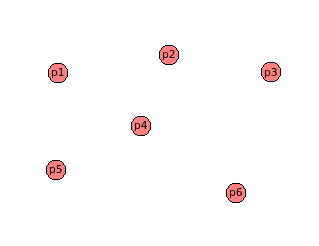
\includegraphics[scale=0.7]{./img/ej2_explicacion1.png}
\caption{Caso trivial}
\end{center}
\end{figure}

Los circulos colorados indican donde fueron instaladas las centrales, en este caso no hay ninguna tuber\'ia.\\

Veamos el siguiente caso mas complejo: 

\begin{figure}[h]
\begin{center}
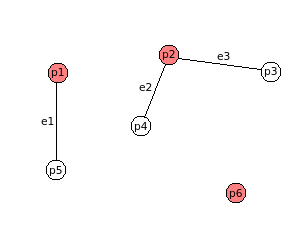
\includegraphics[scale=0.7]{./img/ej2_explicacion2.png}
\caption{Caso con K = 3 y N = 6}
\end{center}
\end{figure}

Como dato, sabemos que $e_2 < e_3 < e_1$ con lo cual nuestro largo m\'aximo de tuber\'ia es $e_1$

\subsection{Resoluci\'on}

Para la resoluci\'on del problema decidimos primero modelarlo con grafos, de forma que los nodos representen los pueblos, y las aristas (con pesos) las posibles conexiones entre pueblos. Los pesos est\'an dados por las distancias entre cada par de pueblos. \\

Como se nos pide minimizar el riesgo de rotura de las tuber\'ias a instalar, lo ideal ser\'ia lograr un esquema de conexiones tal que el largo de la tuber\'ia mas larga sea m\'inimo. Como veremos m\'as adelante, la ubicaci\'on de las centrales de gas no es de gran importancia ya que la transimisi\'on del servicio de gas se da por transitividad entre pueblos conectados (mientras alguno de ellos tenga una central). Por lo tanto lo importante es tener grupos de pueblos conectados a una misma central de manera que las tuber\'as necesarias sean de tama\~no m\'inimo. \\

Para obtener el esquema de conexiones antes mencionado partimos de pensar la regi\'on como un grafo completo; es decir que suponemos que todas las ciudades est\'an conectadas entre s\'i. Luego, a partir del grafo completo la idea es obtener un \'arbol generador m\'inimo del mismo utilizando el algoritmo de Prim.\\
Finalmente cortamos las $k - 1$ aristas m\'as largas del \'arbol, obteniendo un grafo de $k$ componentes conexas tal que la arista m\'as larga del grafo es de peso m\'inimo.\\ 
Como se dijo antes, es indistinto cu\'al de los pueblos de cada componente conexa tiene instalada la central. Sin embargo, como el ejercicio pide especificar el pueblo elegido, instalamos inicialmente una central en la ra\'iz del \'arbol. Luego, por cada arista ($v_1$, $v_2$) que eliminamos instalamos una central en el pueblo representado por $v_2$. %TODO: aclarar por que anda

\subsubsection{Implementaci\'on de Prim}
Describimos a continuaci\'on nuestra implementaci\'on del algoritmo de Prim.\\

Elegimos como ra\'iz del \'arbol generador m\'inimo al primer pueblo de la lista de pueblos de la regi\'on. Como al menos va a haber una central, instalamos una en el pueblo ra\'iz.\\
Luego realizamos un ciclo que se repite $n - 1$ veces (siendo $n$ la cantidad de nodos, es decir, ciudades), en el cual en cada iteraci\'on obtenemos el nodo m\'as cercano al \'arbol y lo agregamos al mismo.\\
Para saber cu\'al es el nodo m\'as cercano al \'arbol debemos, en cada iteraci\'on calcular la distancia m\'inima entre cada nodo que no pertenece al \'arbol y los que s\'i pertenecen.\\
Como partimos de un \'arbol que s\'olo tiene al primer nodo de la lista ($n_0$) inicialmente calculamos la distancia de cada uno de los nodos restantes a $n_0$. Luego se elegimos el nodo de menor distancia y lo agregamos al \'arbol y repetimos el proceso de calcular distancias y elegir el nodo m\'as cercano.\\
As\'i ,cada vez que agregamos un nodo al \'arbol volvemos a computar la m\'inima distancia de los nodos restantes comparando la distancia que cada uno tiene guardada como m\'inima con la distancia al nuevo nodo.\\
Una vez agregados todos los nodos al \'arbol tenemos un \'arbol generador m\'inimo.\\

\subsection{Demostraci\'on de la resoluci\'on}

\subsection{Complejidad del algoritmo}

Veamos la complejidad del algoritmo propuesto utilizando un pseudoc\'odigo que facilite el an\'alisis.\\

Analicemos primero el algoritmo\\

\begin{itemize}
\item poner puebloNuevo $\leftarrow$ primer pueblo de la lista
\item agregar a arbolPueblos $\leftarrow$ (puebloNuevo, puebloNuevo)
\item instalar central en puebloNuevo y poner centralesInstaladas $\leftarrow$ 1
\item poner i $\leftarrow$ 0
\item mientras i < cantidadPueblos - 1 (Agregamos los pueblos uno a uno, n iteraciones)
\begin{itemize}
	\item actualizarDistancias respecto a puebloNuevo (Lo analizamos m\'as adelante, toma O(n))
	\item poner masCercano $\leftarrow$ pueblo mas cercano fuera del arbol
	\item poner cercanoEnArbol $\leftarrow$ pueblo del arbol con el que masCercano tiene distancia minima
	\item agregar arbolPueblos $\leftarrow$ (cercanoEnArbol, masCercano) (Agregar un elemento a una lista es O(1))
\end{itemize}
\item ordenar arbolPueblos de mayor a menor por distancia entre pares 
\item mientras centralesInstaladas < cantidadCentralitas (k iteraciones, que a lo sumo son n)
\begin{itemize}
	\item poner aristaMayor $\leftarrow$ primer elem de arbolPueblos
	\item instalarCentral(aristaMayor.segundo)
	\item eliminar aristaMayor de arbolPueblos (eliminar usando erase es O(1))
\end{itemize}
\end{itemize}

Como se puede ver, la complejidad est\'a dada por el primer ciclo de la implementaci\'on, el cual hace n iteraciones (donde n corresponde a la cantidad de ciudades), ya que debe agregarlas una a una al \'arbol generador m\'inimo. Dentro de ese ciclo se actualizan las distancias de las ciudades al \'arbol; veremos la complejidad de hacerlo a continuaci\'on, pero podemos adelantar que realiza n iteraciones tambi\'en.\\
Una vez obtenido el \'arbol lo ordenamos de mayor a menor, donde el par ($v_1$, $v_2$) es mayor a otro ($w_1$, $w_2$) si la distancia entre $v_1$ y $v_2$ es mayor a la distancia entre $w_1$ y $w_2$. Ordenar una lista con std::list::sort toma O(n*log(n)).\\
Finalmente eliminamos los primeros k-1 (donde k es el n\'umero de centrales) pares de pueblos; es decir los pares que tienen mayor distancia. Esto toma O(k) que es, a lo sumo O(n).\\

Vemos ahora el pseudoc\'odigo de actualizarDsitancias para confirmar que es O(n).\\

%Por el for anidado que tenemos, que nos lleva a recorrer dos veces la lista de pueblos, obtenemos una complejidad de $O(n^2)$

\newpage

\subsection{C\'odigo fuente}

\lstset{language=C++,
                basicstyle=\ttfamily\footnotesize,
                keywordstyle=\color{blue}\ttfamily,
                stringstyle=\color{red}\ttfamily,
                commentstyle=\color{green}\ttfamily,
                morecomment=[l][\color{magenta}]{\#},
                breaklines=true
}
\begin{lstlisting}

/* Constructor de region */
Region::Region(list<Pueblo*> * lista_pueblos, int centralitas){
	
	_centralitas = centralitas;
	_centrales_instaladas = 0;
	_tuberias_instaladas = 0;
	_pueblos = lista_pueblos;
	_arbol_pueblos = new list<pair<Pueblo*, Pueblo*> >();

}

void Region::resolver(){

	int cantPueblos = _pueblos->size();
	
	// Uso Prim para agregar pueblos al arbol

	// Elijo la primera ciudad de la lista como root
	Pueblo* puebloNuevo = *_pueblos->begin();
	pair<Pueblo*, Pueblo*> parPueblos = pair<Pueblo*, Pueblo*>(puebloNuevo, puebloNuevo);
	_arbol_pueblos->push_back(parPueblos);
	// Inicialmente solo el pueblo root tiene una central instalada
	puebloNuevo->instalarCentral();
	_centrales_instaladas = 1;

	// Pueblo mas cercano actual
	Pueblo * masCercano = puebloNuevo;

	// Agrego ciudades al arbol de a una - O(n)
	for(int i=0; i<cantPueblos-1 ; i++){
		
		// Actualizo las distancias al arbol y me quedo con la menor
		//cout << "nuevo_id: " << puebloNuevo->getId() << endl;
		masCercano = actualizarDistancias(puebloNuevo);

		// Agrego masCercano al arbol
		// En la proxima iteracion la distancia va a quedar en 0
		parPueblos = pair<Pueblo*, Pueblo*>(masCercano->getPuebloCercano(), masCercano);
		_arbol_pueblos->push_back(parPueblos);
		puebloNuevo = masCercano;
	}

	// Ordeno los pares de ciudades segun distancia (de mayor a menor)
	_arbol_pueblos->sort(compararDistancia);

	// Mientras que pueda instalar centrales achico el tam maximo de las tuberias
	// Es decir, genero k componentes conexas, cada una con una central

	for(list<pair<Pueblo*,Pueblo*> >::iterator p = _arbol_pueblos->begin(); p != _arbol_pueblos->end(); p++){
		if(_centrales_instaladas<_centralitas){
			// p representa la tuberia mas larga, la elimino e instalo una nueva central
			((*p).second)->instalarCentral();
			_centrales_instaladas++;
			_arbol_pueblos->erase(p++);
		}	
	}

	printPueblosConectados();	
}

// Actualiza distancia minima al arbol de cada pueblo y devuelve el mas cercano
Pueblo* Region::actualizarDistancias(Pueblo* puebloNuevo){

	double distActual;
	double distNueva;
	double min = std::numeric_limits<double>::infinity();
	Pueblo* masCercano = puebloNuevo;

	// Antes de empezar actualizo la distancia del nuevo pueblo
	puebloNuevo->setDistanciaArbol(0.0);

	// Recorro todos los pueblos y actualizo sus distancias al arbol comparando con el ultimo p agregado
	for(list<Pueblo*>::iterator p = _pueblos->begin(); p != _pueblos->end(); p++){

		distActual = (**p).getDistanciaArbol();

		// Si no pertenece al arbol actualizo
		if(distActual > 0.0){

			distNueva = (**p).distancia(*puebloNuevo);
			
			if(distNueva < distActual){
				(**p).setPuebloCercano(puebloNuevo);
				(**p).setDistanciaArbol(distNueva);
			}

			distActual = (**p).getDistanciaArbol();

			// Si es el menor hasta el momento guardo la ciudad
			if(distActual < min){
				masCercano = *p;
			}
		}
	
	}

	return masCercano;
}

\end{lstlisting}

\subsection{Casos de prueba}

\subsection{Performance}
